\documentclass{article}

\usepackage{graphicx}
\usepackage{tikz}
\usepackage{tikzsymbols}
\usetikzlibrary{calc,patterns,shapes.geometric}
\pagestyle{empty}
\usepackage[margin=0pt]{geometry}
\geometry{papersize={14in,12in}}

\def\centerarc[#1](#2)(#3:#4:#5){\draw[#1] ($(#2)+({#5*cos(#3)},{#5*sin(#3)})$) arc (#3:#4:#5);}

\begin{document}
	\begin{figure}
		\centering
		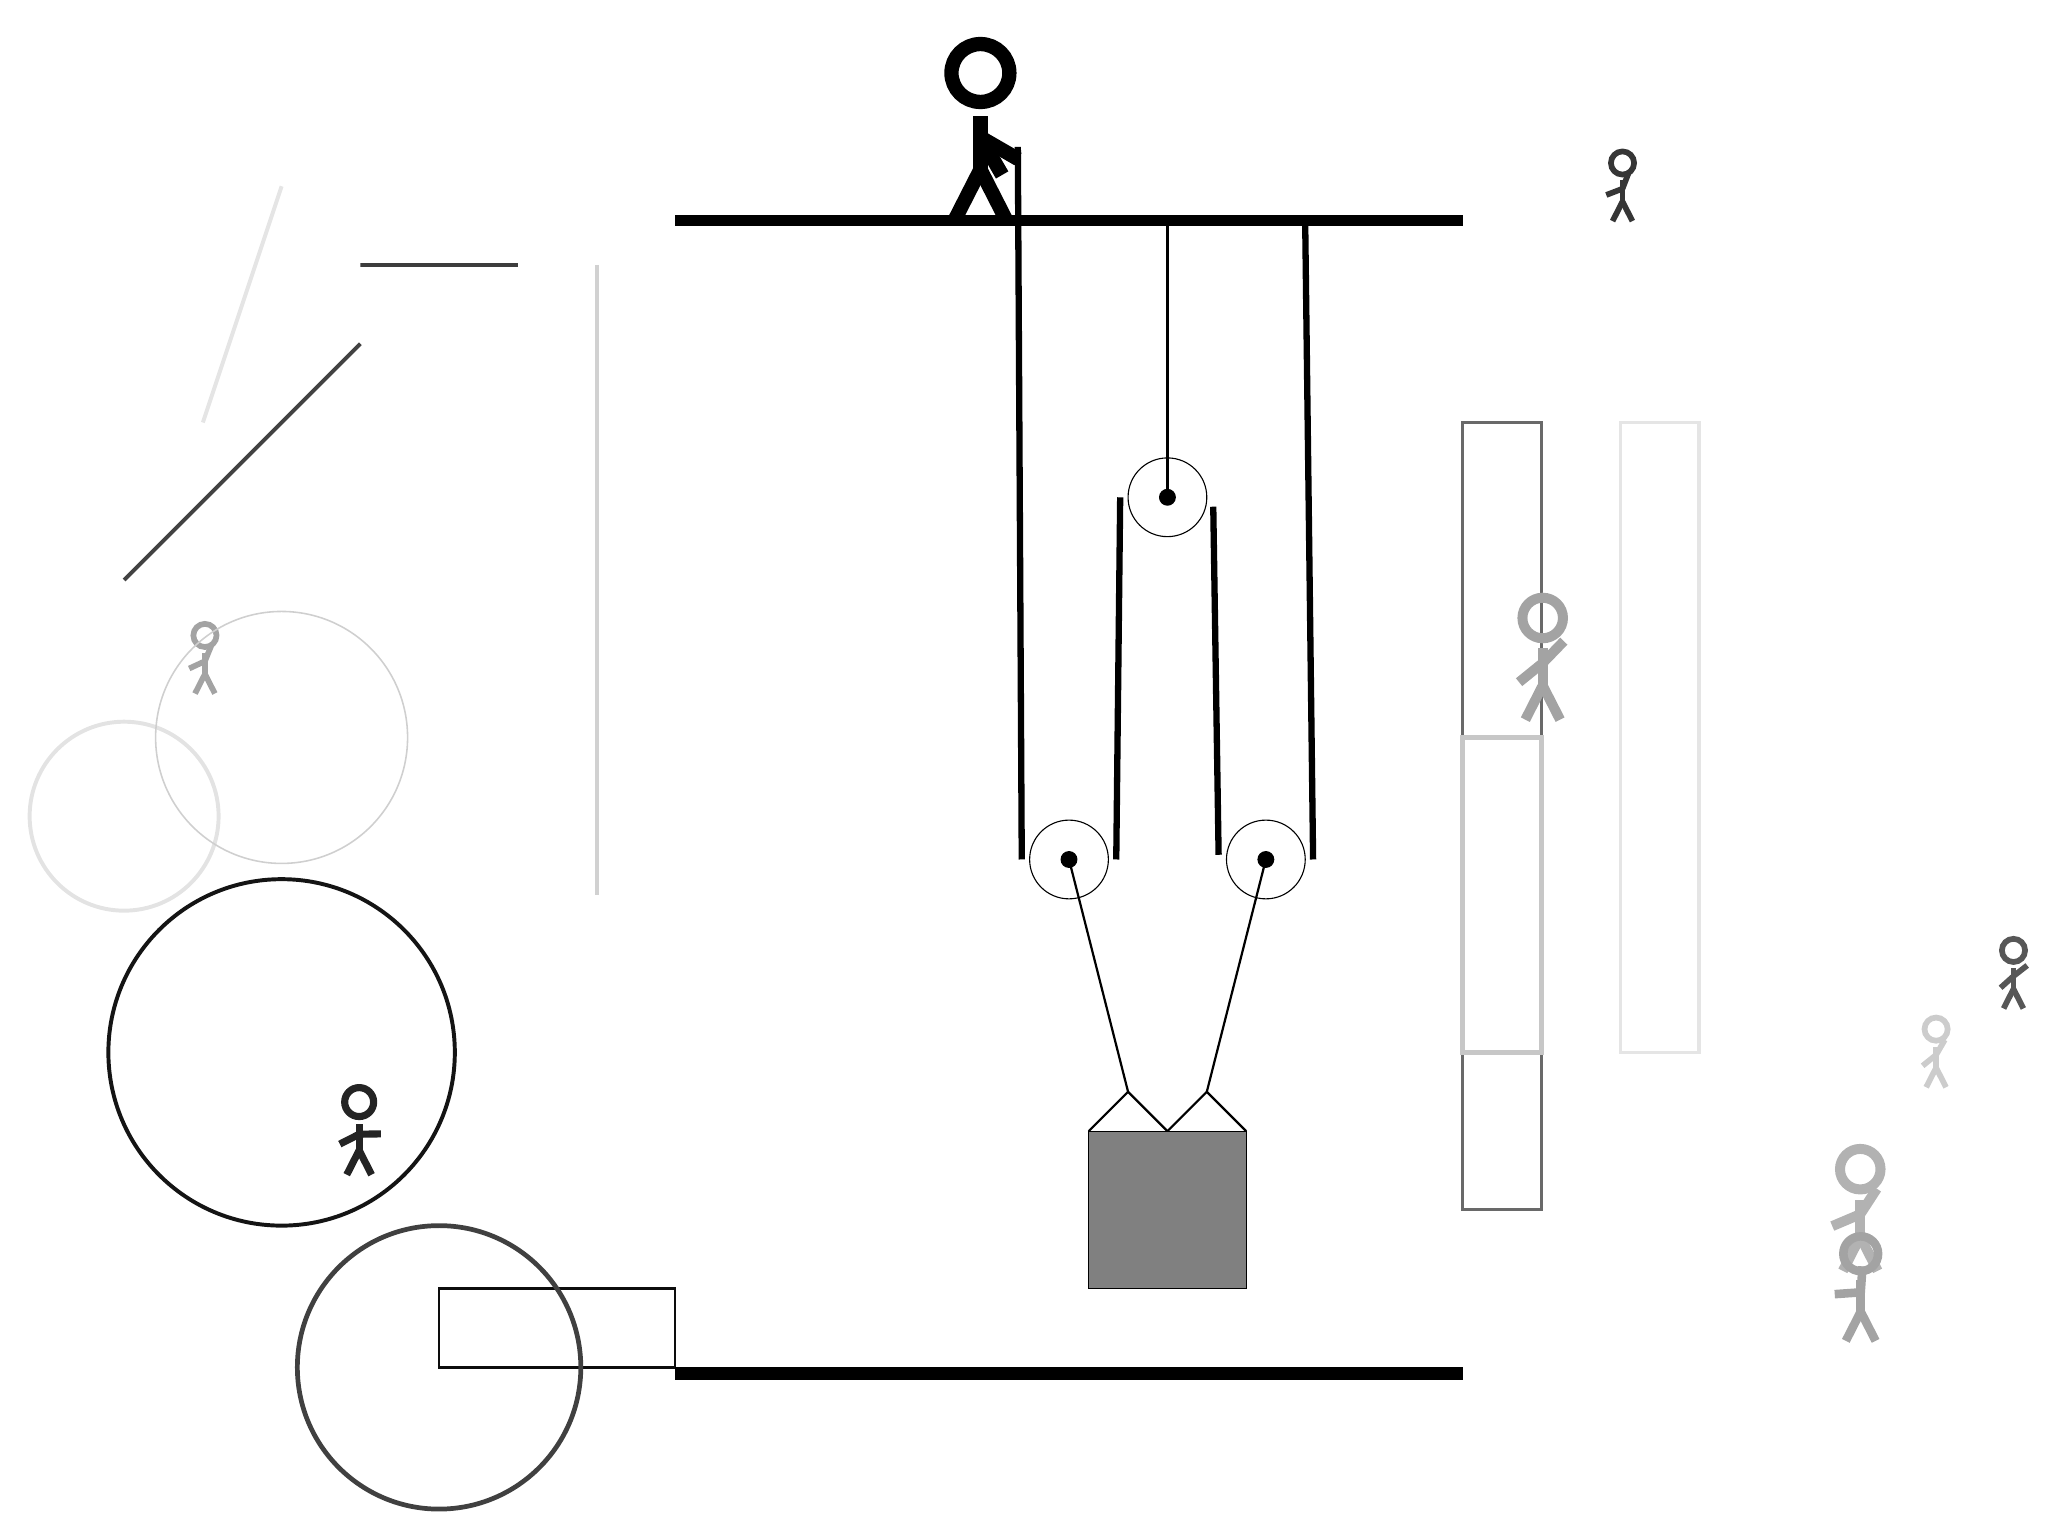
\begin{tikzpicture}
			%%%%% START %%%%%
			
			\draw[fill=black] (-4, 11.5) rectangle (6, 11.625);
			
			\draw (1, 3.45) circle (0.5);
			\draw[fill=black] (1, 3.45) circle (0.1);
			
			\draw (2.25, 8.05) circle (0.5);
			\draw[fill=black] (2.25, 8.05) circle (0.1);
			\draw[thick] (2.25, 8.05) -- (2.25, 11.5);
			
			\draw (3.5, 3.45) circle (0.5);
			\draw[fill=black] (3.5, 3.45) circle (0.1);
			
			\draw[thick] (3.5, 3.45) -- (2.75, 0.5);
			\draw[thick] (1, 3.45) -- (1.75, 0.5);
			\draw[thick]  (1.25, 0) -- (1.75, 0.5) -- (2.25, 0);
			\draw[thick]  (2.25, 0) -- (2.75, 0.5) -- (3.25, 0);
			\draw[fill=black!50] (1.25, 0) rectangle (3.25, -2);
			
			\node[line width=0.5mm, color=black!20] at (12, 1) {\Strichmaxerl[4][39][60]};
			
			\draw[line width=0.3mm, color=black!95] (-4, -2) rectangle (-7, -3);
			\draw[line width=0.4mm, color=black!59] (7, -1) rectangle (6, 9);
			\node[line width=0.7mm, color=black!79] at (8, 12) {\Strichmaxerl[4][21][69]};
			
			\draw[line width=0.5mm, color=black!74](-8, 10) -- (-11, 7);
			\node[line width=0.7mm, color=black!30] at (11, -1) {\Strichmaxerl[7][23][57]};
			\draw [line width=0.5mm, color=black!92](-9, 1) circle (2.2);
			\draw[line width=0.5mm, color=black!10](-9, 12) -- (-10, 9);
			\draw [line width=0.2mm, color=black!39](13, 9) circle (0.0);
			\draw[line width=0.5mm, color=black!18](-5, 11) -- (-5, 3);
			
			\node[line width=0.7mm, color=black!36] at (11, -2) {\Strichmaxerl[6][4][86]};
			
			\draw [line width=0.6mm, color=black!75](-7, -3) circle (1.8);
			\draw[line width=0.6mm, color=black!22] (6, 1) rectangle (7, 5);
			
			\draw[line width=0.4mm, color=black!10] (8, 1) rectangle (9, 9);
			\node[line width=0.3mm, color=black!86] at (-8, 0) {\Strichmaxerl[5][27][1]};
			\draw [line width=0.5mm, color=black!11](-11, 4) circle (1.2);
			\node[line width=0.4mm, color=black!36] at (-10, 6) {\Strichmaxerl[4][25][68]};
			\node[line width=0.7mm, color=black!36] at (7, 6) {\Strichmaxerl[7][39][46]};
			\draw [line width=0.2mm, color=black!19](-9, 5) circle (1.6);
			\draw[line width=0.5mm, color=black!76] (-6, 11) rectangle (-8, 11);
			\node[line width=0.5mm, color=black!66] at (13, 2) {\Strichmaxerl[4][42][38]};
			
			\draw[line width=0.8mm] (0.35, 12.5) --  (0.4, 3.45);
			\centerarc[line width=0.8mm](1, 3.45)(180:360:0.6);
			\draw[line width=0.8mm] (1.6, 3.45) -- (1.65, 8.05);
			\centerarc[line width=0.8mm](2.25, 8.05)(-20:180:0.6);
			\draw[line width=0.8mm](2.832, 7.93) -- (2.9, 3.51);
			\centerarc[line width=0.8mm](3.5, 3.45)(160:360:0.6);
			\draw[line width=0.8mm](4.1, 3.45) -- (4.0, 11.5);
			
			\node at (-0.07, 12.7) {\Strichmaxerl[10][120][-30]};
			
			\draw[fill=black] (-4, -3) rectangle (6, -3.15);
			
			%%%%% END %%%%%
		\end{tikzpicture}
	\end{figure}	
\end{document}